\lecture{1}{mardi 04 février 2020}
\vspace{-1.2cm}

\section{Introduction au cours}

Qu'est-ce que l'ingénierie linguistique? Le nom de ce cours est ancien, aujourd'hui on dirait plutôt
"Introduction au Traitement Automatique des Langues (TAL)". On garde cet ancien nom car il est
intéressant (il mets en évidence qu'il s'agit d'un mix entre sciences "dures" et sciences "sociales"). \\

Il s'agit d'une discipline en constante évolution et hybride. Historiquement, deux disciplines dissociées et
ayant des chercheurs distincts existaient: d'un coté des linguistes s'interrogeant sur ce que l'informatique
pourrait apporter à leur discipline (linguistique informatique), et de l'autre des informaticiens et ingénieurs
curieux d'appliquer leurs modèles mathématiques dans l'étude de la linguistique (traitement automatique des langues).
À présent, les deux disciplines sont communes. \\

\textbf{Applications possibles de la discipline:}\\

\begin{minipage}[t]{0.6\textwidth}
\begin{itemize}
\item Correction orthographique/grammaticale
\item Traduction automatique/assistée
\item Reconnaissance et synthèse vocale
\end{itemize}
\end{minipage}
\begin{minipage}[t]{0.4\textwidth}
\begin{itemize}
\item Extraction d'informations
\item Analyse de sentiments
\item Question answering
\end{itemize}
\end{minipage}

\subsection{Niveaux linguistiques}

\begin{figure}[H]
\centering
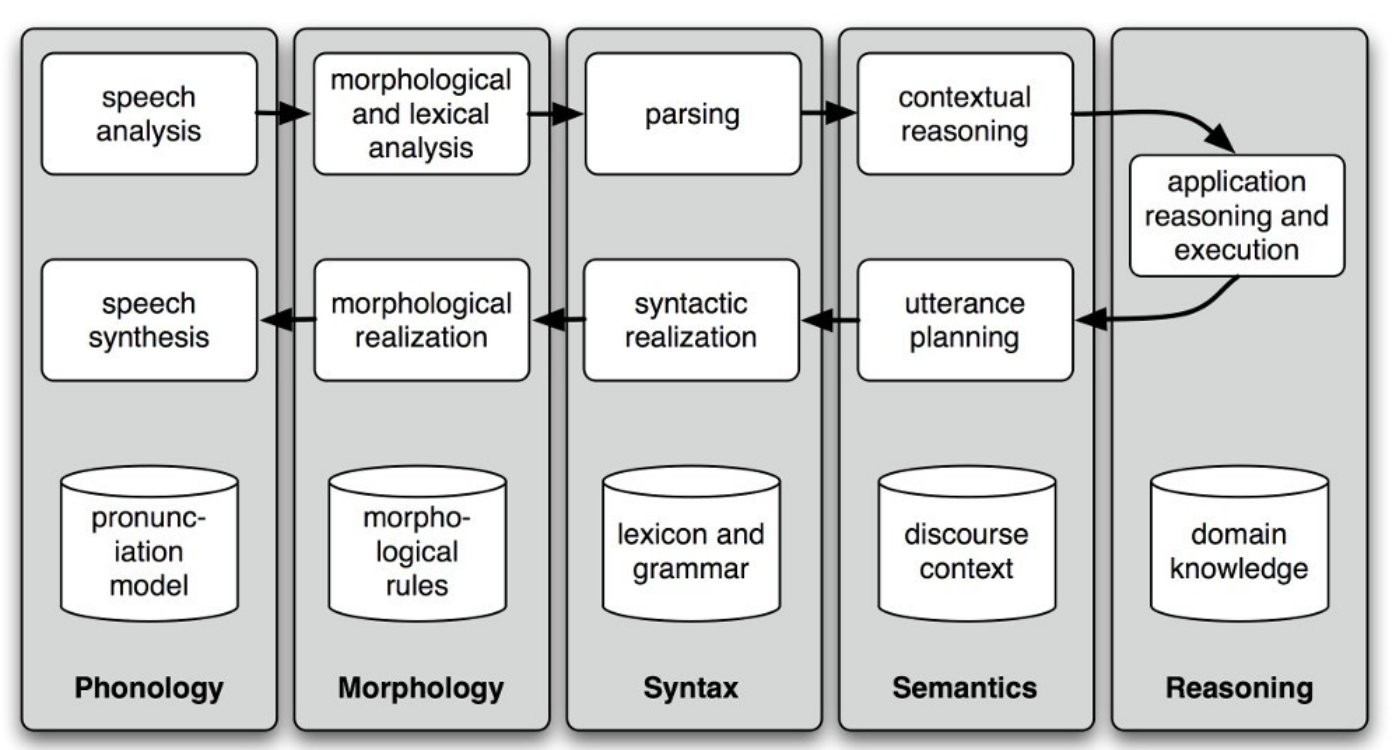
\includegraphics[scale=0.25]{lec1img1}
\end{figure}

Dans ce cours on étudie les nombreux niveaux linguistiques existants et les challenges qu'ils apportent au niveau
de l'ingénierie linguistique, car le langage humain est ambigu à tous les niveaux.\\

\begin{itemize}
    \item \textbf{Phonétique / Phonologie}: Hors scope du cours. Reconnaissance de mots depuis un signal audio et
    génération d'un signal audio à partir de mots. Prononciation, réalisation acoustique, etc.
    \item \textbf{Morphologie}: Reconnaissance des variations de forme des mots individuels (pluriel, conjugaison,...).
    \item \textbf{Lexique}: Qu'est-ce qu'un mot? Il faut savoir comment découper une phrase en mots pour la traiter par la suite.
    \item \textbf{Syntaxe}: Reconnaissance de l'ordre des mots et de l'organisation interne d'une phrase structurée.
    \item \textbf{Sémantique}: Reconnaissance du sens intrinsèque des mots (sémantique lexicale) ainsi que de la manière dont
    ils s'influencent mutuellement (sémantique compositionnelle).
    \item \textbf{Pragmatique}: Brièvement discuté lors du cours, mais hors scope du cours. Reconnaissance de l'intention du
    locuteur de la manière appropriée d'y répondre en fonction du contexte.
\end{itemize}

\subsection{Challenges affrontés}

\textbf{Ambigüités possibles:}

\begin{itemize}
    \item \textbf{Ambigüité phonétique}: Homophonie
    \item \textbf{Ambigüité morpho-lexicale}: Homographie
    \item \textbf{Ambigüité syntaxique}
    \item \textbf{Ambigüité sémantique} Hors contexte, certaines phrases peuvent être lues de façons différentes
    \item \textbf{Ambigüité pragmatique}: Ironie, par exemple
    \item \textbf{Ambigüité multilingue} \\
\end{itemize}

\noindent\textbf{Contraintes supplémentaires:}

\begin{itemize}
    \item \textbf{Précision}: Reproduire la compétence linguistique des êtres humains à l'aide de modèles
    formalisant notre compréhension
    \item \textbf{Rappel}: Une bonne couverture de la langue traitée requiert des ressources
    linguistiques (lexiques, grammaires,...) suffisamment fournies
    \item \textbf{Performance}: Un traitement rapide implique de limiter la complexité des modèles linguistiques
\end{itemize}

\subsection{Un peu d'histoire}

\textbf{Hiérarchie de Noam Chomsky (1956)} \\

Classification des grammaires en quatre catégories, de la plus libre à la plus contraignante

\vspace{1cm}

\resizebox{0.9\textwidth}{!}{
    


\tikzset{every picture/.style={line width=0.75pt}} %set default line width to 0.75pt

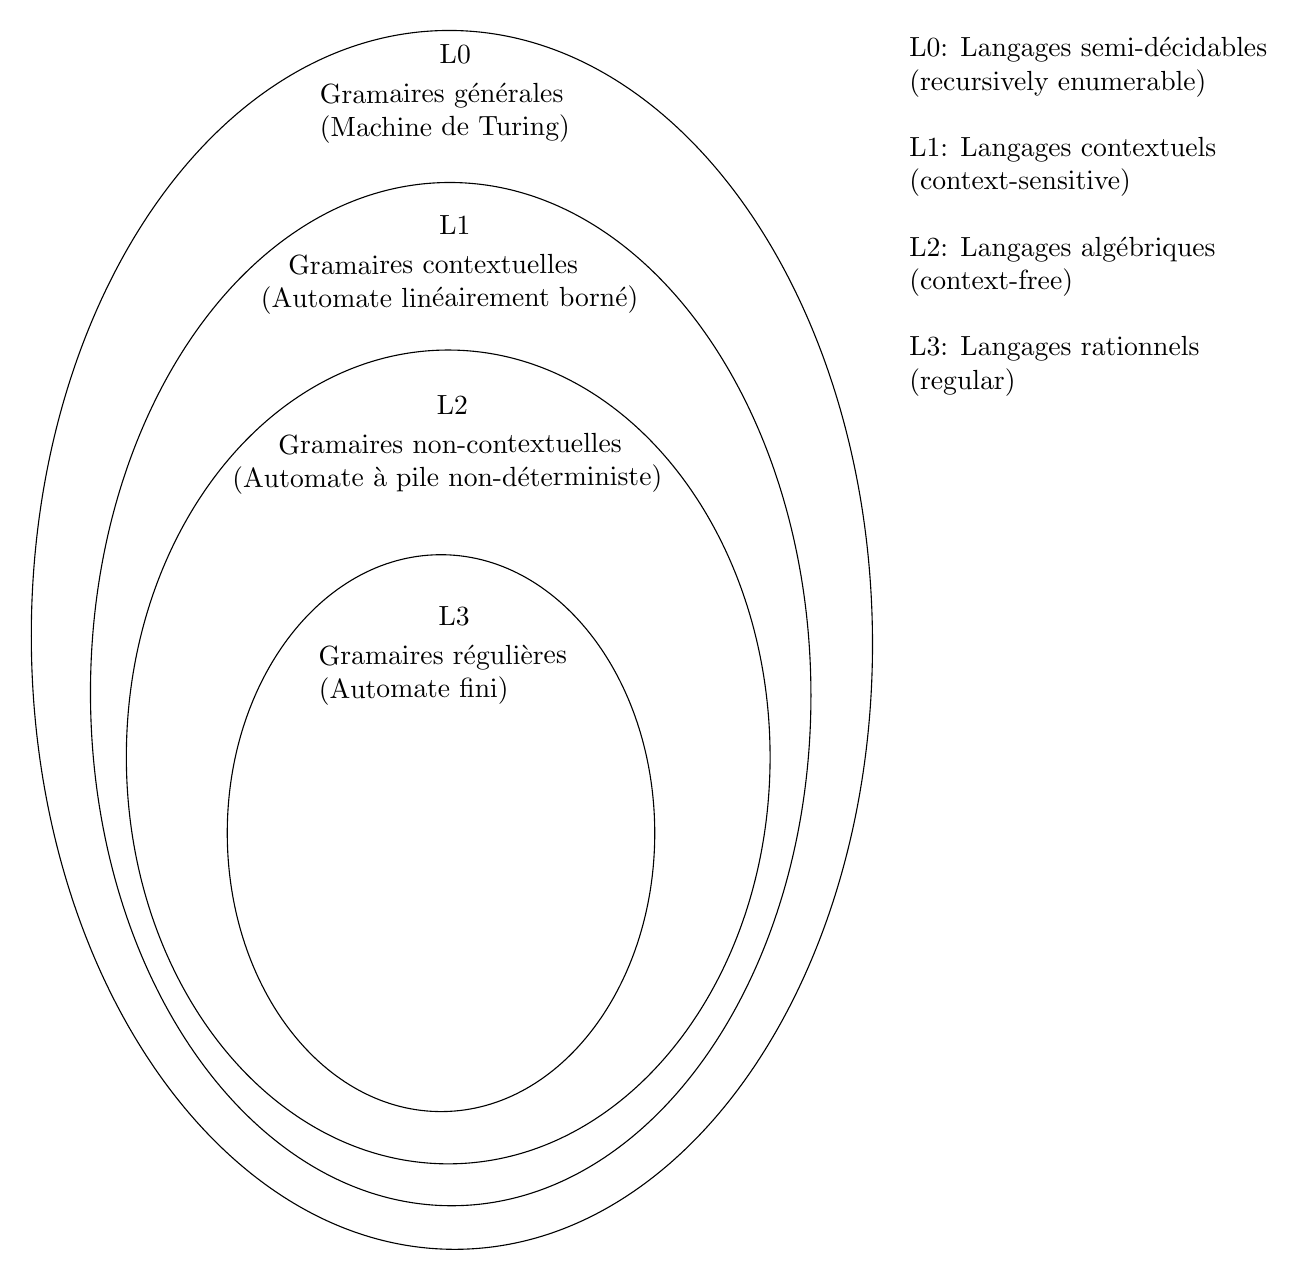
\begin{tikzpicture}[x=0.75pt,y=0.75pt,yscale=-1,xscale=1]
%uncomment if require: \path (0,777); %set diagram left start at 0, and has height of 777

%Shape: Ellipse [id:dp589513737865884]
\draw   (212.11,6.76) .. controls (324.01,5.68) and (415.95,136.27) .. (417.45,298.43) .. controls (418.95,460.59) and (329.45,592.92) .. (217.54,593.99) .. controls (105.63,595.07) and (13.7,464.48) .. (12.2,302.32) .. controls (10.7,140.16) and (100.2,7.83) .. (212.11,6.76) -- cycle ;
%Shape: Ellipse [id:dp20608648020649545]
\draw   (212.36,80.01) .. controls (308.21,78.91) and (386.76,188.37) .. (387.8,324.5) .. controls (388.85,460.63) and (311.99,571.88) .. (216.14,572.99) .. controls (120.29,574.09) and (41.75,464.63) .. (40.7,328.5) .. controls (39.66,192.37) and (116.51,81.11) .. (212.36,80.01) -- cycle ;
%Shape: Ellipse [id:dp9918973051483866]
\draw   (211.57,160.73) .. controls (297.22,159.72) and (367.3,246.68) .. (368.12,354.95) .. controls (368.93,463.22) and (300.16,551.8) .. (214.52,552.81) .. controls (128.88,553.81) and (58.79,466.85) .. (57.98,358.58) .. controls (57.16,250.31) and (125.93,161.73) .. (211.57,160.73) -- cycle ;
%Shape: Ellipse [id:dp8223736553004263]
\draw   (208.59,259.34) .. controls (265.47,258.67) and (312.01,318.18) .. (312.55,392.26) .. controls (313.1,466.35) and (267.43,526.96) .. (210.56,527.63) .. controls (153.69,528.31) and (107.14,468.8) .. (106.6,394.71) .. controls (106.05,320.62) and (151.72,260.02) .. (208.59,259.34) -- cycle ;

% Text Node
\draw (149.79,12.8) node [anchor=north west][inner sep=0.75pt]  [rotate=-359.73] [align=left] {\begin{minipage}[lt]{98.022pt}\setlength\topsep{0pt}
\begin{center}
L0
\end{center}
Gramaires générales\\(Machine de Turing)
\end{minipage}};
% Text Node
\draw (433.93,9) node [anchor=north west][inner sep=0.75pt]   [align=left] {L0: Langages semi-décidables\\(recursively enumerable)\\\\L1: Langages contextuels\\(context-sensitive)\\\\L2: Langages algébriques\\(context-free)\\\\L3: Langages rationnels\\(regular)};
% Text Node
\draw (121.26,95.32) node [anchor=north west][inner sep=0.75pt]  [rotate=-359.73] [align=left] {\begin{minipage}[lt]{140.57844pt}\setlength\topsep{0pt}
\begin{center}
L1
\end{center}
 \ \ \ Gramaires contextuelles\\(Automate linéairement borné)
\end{minipage}};
% Text Node
\draw (107.59,181.9) node [anchor=north west][inner sep=0.75pt]  [rotate=-359.73] [align=left] {\begin{minipage}[lt]{159.29000000000002pt}\setlength\topsep{0pt}
\begin{center}
L2
\end{center}
 \ \ \ \ \ Gramaires non-contextuelles\\ \ \ (Automate à pile non-déterministe)
\end{minipage}};
% Text Node
\draw (149.22,283.45) node [anchor=north west][inner sep=0.75pt]  [rotate=-359.73] [align=left] {\begin{minipage}[lt]{98.01044000000002pt}\setlength\topsep{0pt}
\begin{center}
L3
\end{center}
Gramaires régulières\\ \ \ \ (Automate fini)
\end{minipage}};


\end{tikzpicture}

}

\newpage

\textbf{Test de Turing / Imitation Game} \\

Proposition de test d'intelligence artificielle décrit par Alan Turing en 1950. Ce test consiste à mettre un humain en conversation à l'aveugle avec un ordinateur et un autre humain pour évaluer la capacité de cette machine à imiter la conversation humaine. Si le programme réussis à tromper des humains plus de 30\% des fois, on considère le test réussi. \\

De nombreuses objections à ce test ont été suggérées tout comme réfutées depuis des années, certaines par Alan Turing lui-même, mais il reste tout de même un théorème central dans l'étude de l'intelligence artificielle. \\

ELIZA, une simulation de thérapie rogérienne développée en 1966, a été une des premières à tromper des humains mais on peut pas dire qu'il s'agit d'un succès du test de Turing, car les personnes l'utilisant n'avaient aucune raison de suspecter qu'elles ne parlaient pas à un humain, ce qui est l'élément central du test. \\

\subsection{Éclatement de la discipline}

\textbf{Approches linguistiques}

Aussi appelées symboliques ou rule-based. Basées sur la compréhension du langage et
l'intuition humaine. Patterns récurrents + heuristiques simples.
Nécessitent de coder chaque règle à la main : investissement énorme en termes de temps, argent et ressources humaines \\

\textbf{Approches statistiques}

Aussi appelées stochastiques ou probabilistes. Très rapides mais souvent moins précises.

Modèle bayésien naïf : inférence permettant d'estimer la probabilité d'une chaîne de caractères à partir des probabilités de chaînes existantes. \\

\textbf{Approches hybrides}

Combinent la puissance des approches statistiques avec la finesse d'analyse des approches linguistiques.
La plupart des systèmes actuels sont de ce type et incluent donc différentes composantes complémentaires pour atteindre un niveau de pointe. \\

\textbf{Apprentissage automatique}

Plus connu sous le nom de machine learning. Data-driven : nécessite un grand volume de
données pour entraîner les algorithmes.

Utilisation de corpus annotés : Penn Treebank, Brown, Reuters, Europarl...

Supervisé vs non-supervisé. Apprentissage profond (deep learning) et réseaux de neurones.

\subsection{État de l'art}

\textbf{Globalement résolu}

Détéction de spam. Tagging the part-of-speech. "Named entity recognition" (NER).\\

\textbf{En progrès constant}

Analyse de sentiment de texte. Parsing. Traduction automatique. Extraction d'information.\\

\textbf{Toujours très complexe}

Question answering. Paraphrase. Résumé de texte. Dialogue.\\
